\documentclass[conference]{IEEEtran}
\IEEEoverridecommandlockouts

\usepackage{cite}
\usepackage{amsmath,amssymb,amsfonts}
\usepackage{graphicx}
\usepackage{textcomp}
\usepackage{xcolor}
\usepackage{tikz}
\usetikzlibrary{shapes,arrows,arrows.meta,positioning,calc,fit}
\usepackage{url}
\usepackage{hyperref}

\hypersetup{
    colorlinks=true,
    linkcolor=blue,
    citecolor=blue,
    urlcolor=blue
}

\def\BibTeX{{\rm B\kern-.05em{\sc i\kern-.025em b}\kern-.08em
    T\kern-.1667em\lower.7ex\hbox{E}\kern-.125emX}}

\begin{document}

\title{Real-Time Vibration Suppression of a Flexible Beam Using Active Disturbance Rejection Control (ADRC)}

\author{
\IEEEauthorblockN{Niya Rachel Juban}
\IEEEauthorblockA{\textit{Dept. of Electronics \& Communication Eng.} \\
\textit{Vellore Institute of Technology}\\
Vellore, India \\
niya.racheljuban2024@vitstudent.ac.in}
\and
\IEEEauthorblockN{Swathi C P}
\IEEEauthorblockA{\textit{Dept. of Electronics \& Communication Eng.} \\
\textit{Vellore Institute of Technology}\\
Vellore, India \\
swathi.cp2024@vitstudent.ac.in}
\and
\IEEEauthorblockN{Aparajita Yarramsetti}
\IEEEauthorblockA{\textit{Dept. of Electronics \& Communication Eng.} \\
\textit{Vellore Institute of Technology}\\
Vellore, India \\
aparajita.2024@vitstudent.ac.in}
\and
\IEEEauthorblockN{Disha Devarmani}
\IEEEauthorblockA{\textit{Dept. of Electronics \& Communication Eng.} \\
\textit{Vellore Institute of Technology}\\
Vellore, India \\
disha.devarmani2024@vitstudent.ac.in}
}

\maketitle

\begin{abstract}
Lightweight flexible arms and compliant link mechanisms are increasingly utilized in precision robotics, automated gantries, and aerospace appendages due to their high payload-to-weight ratio and low power requirements. However, rapid actuator slewing and point-to-point step movements induce severe vibrations due to structural compliance and low inherent material damping. Conventional control methodologies, such as proportional-integral-derivative (PID) control or open-loop input shaping, suffer from derivative sensor noise amplification, phase lag, and vulnerability to boundary-condition stiffness variations. In this paper, a Linear Active Disturbance Rejection Control (LADRC) framework is formulated, physically constructed, and experimentally validated to achieve real-time vibration suppression. The experimental testbed incorporates a 12V DC motor, a circular plastic wheel hub, a commercial 30~cm flexible plastic scale as the cantilever beam, a tip-mounted MPU-6050 accelerometer, an L298N H-bridge driver, and an ESP32 microcontroller running a deterministic 200~Hz discrete loop. By abstracting structural elasticity, high-order bending modes, and motor friction into a single unified ``Total Disturbance,'' a second-order Linear Extended State Observer (LESO) in the acceleration domain reconstructs and cancels the flexural disturbance forces in real time. Experimental trials verify that while an uncontrolled step exhibits aggressive initial whipping and prolonged ringing, the introduction of LADRC actively drains kinetic energy from the flexural mode, delivering rapid oscillation damping and swift stabilization.
\end{abstract}

\begin{IEEEkeywords}
Active Disturbance Rejection Control (ADRC), Linear Extended State Observer (LESO), Flexible Beam, Vibration Suppression, ESP32, MPU-6050, Embedded Control.
\end{IEEEkeywords}

\section{Introduction}
Modern industrial automation, high-speed pick-and-place robots, and deployable space structures increasingly prioritize lightweight materials to minimize energy consumption and achieve rapid maneuvering speeds \cite{dwivedy2006dynamic}. However, reduced mass inevitably sacrifices structural rigidity. When an actuator commands an abrupt step displacement to the base of a flexible link, the inertia of the beam causes the tip to lag behind, storing potential strain energy. Upon actuator deceleration, this stored strain energy releases, initiating a sequence of violent whips and sustained residual oscillations \cite{krauss2019vibration}.

Historically, two broad paradigms have been deployed to mitigate these vibrations:
\begin{enumerate}
    \item \textbf{Feedforward Input Shaping:} Techniques such as Zero Vibration (ZV) preshape actuator inputs into a series of delayed impulses to induce destructive interference at specific modal frequencies \cite{singer1990preshaping}. While computationally simple, input shaping is strictly open-loop; any parametric variation in beam length, payload mass, or root clamping elasticity degrades the notch filter, leaving residual vibrations unmitigated.
    \item \textbf{Classical Feedback (PID) and Modern Robust Control:} Proportional-Integral-Derivative (PID) control requires aggressive derivative gains ($K_d$) to introduce virtual damping. On physical hardware, discrete numerical differentiation of micro-electro-mechanical systems (MEMS) accelerometer data severely amplifies high-frequency measurement noise, generating actuator chatter. Conversely, modern robust controllers ($H_\infty$, Linear Quadratic Regulators) mandate high-fidelity distributed-parameter models (e.g., Euler-Bernoulli or Timoshenko formulations) that are difficult to calibrate across varying operating temperatures and motor joint backlash \cite{ge1998model}.
\end{enumerate}

To overcome the dichotomy between open-loop sensitivity and model-dependent complexity, Active Disturbance Rejection Control (ADRC), pioneered by Han \cite{han2009pid} and formalized with bandwidth parameterization by Gao \cite{gao2003scaling}, presents an intuitive, model-free alternative. Instead of attempting to model complex structural dynamics, ADRC lumps internal flexural forces, material damping uncertainties, aerodynamic resistance, and actuator nonlinearities into an unmeasured, generalized state termed the \textbf{Total Disturbance}. An Extended State Observer (ESO) estimates this disturbance in real time, allowing the controller to actively compensate for it and decouple the physical plant into an idealized cascaded integrator system \cite{zheng2012active, madonski2019active}.

This work details the theoretical derivation, firmware architecture, and experimental realization of an acceleration-domain LADRC pipeline implemented on an ultra-low-cost embedded platform.

\begin{figure*}[t]
\centering
\IfFileExists{adrc_block_diagram.png}{%
  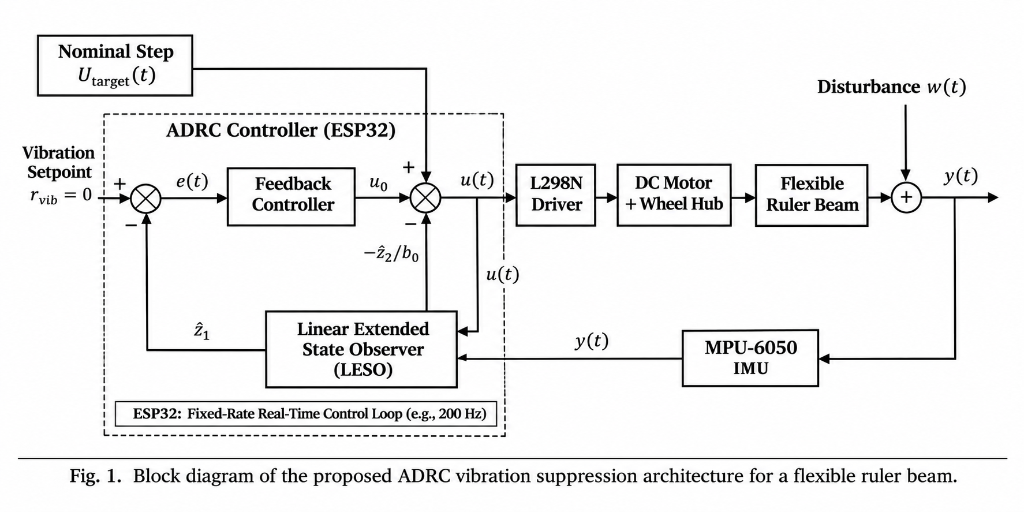
\includegraphics[width=0.92\textwidth]{adrc_block_diagram.png}%
}{%
  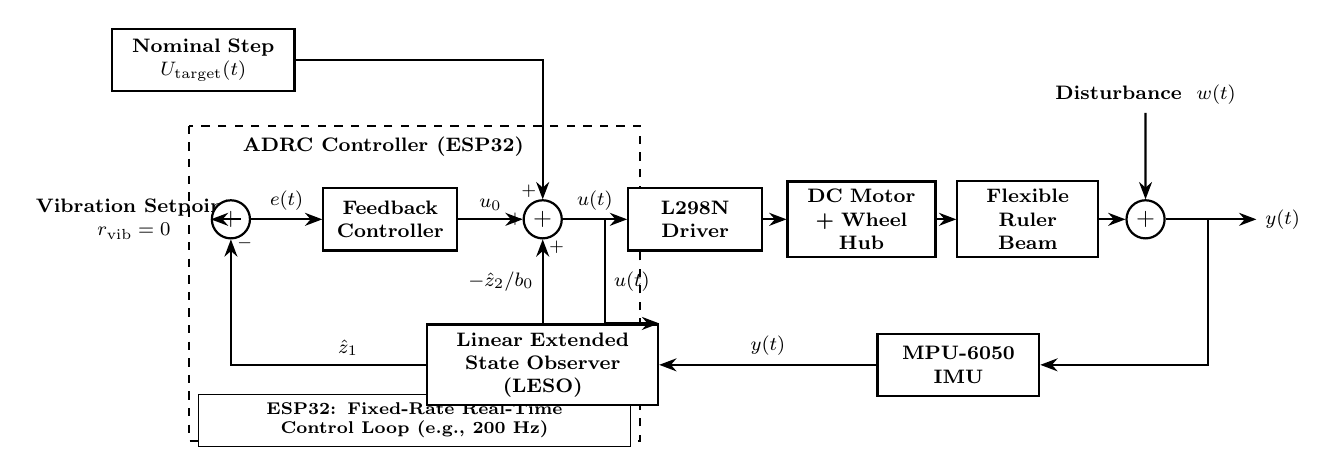
\begin{tikzpicture}[
    scale=0.88, every node/.style={transform shape},
    block/.style={rectangle, draw, thick, fill=white, text width=1.7cm, minimum height=0.9cm, align=center, font=\footnotesize},
    bigblock/.style={rectangle, draw, thick, fill=white, text width=3.1cm, minimum height=1.0cm, align=center, font=\footnotesize},
    sum/.style={circle, draw, thick, fill=white, minimum size=5.5mm, inner sep=0pt},
    arrow/.style={-{Stealth[length=2.2mm]}, thick},
    line/.style={thick}
  ]
    % Outer dashed container
    \draw[dashed, thick] (0.1, 1.35) rectangle (6.6, -3.2);
    \node at (2.9, 1.05) [font=\footnotesize\bfseries] {ADRC Controller (ESP32)};
    \node[draw, solid, thin, fill=white, font=\scriptsize\bfseries, text width=6.0cm, align=center] at (3.35, -2.9) {ESP32: Fixed-Rate Real-Time Control Loop (e.g., 200 Hz)};

    % Top nominal step
    \node[block, text width=2.4cm] (nom) at (0.3, 2.3) {\textbf{Nominal Step}\\ $U_{\text{target}}(t)$};

    % Vibration setpoint
    \node (sp) at (-0.7, 0) [align=center, font=\footnotesize] {\textbf{Vibration Setpoint}\\ $r_{\text{vib}} = 0$};

    % Nodes on main path
    \node[sum] (sum1) at (0.7, 0) {+};
    \node[block] (ctrl) at (3.0, 0) {\textbf{Feedback}\\\textbf{Controller}};
    \node[sum] (sum2) at (5.2, 0) {+};
    \node[block] (l298n) at (7.4, 0) {\textbf{L298N}\\\textbf{Driver}};
    \node[block, text width=1.9cm] (motor) at (9.8, 0) {\textbf{DC Motor}\\ \textbf{+ Wheel Hub}};
    \node[block, text width=1.8cm] (beam) at (12.2, 0) {\textbf{Flexible}\\ \textbf{Ruler Beam}};
    \node[sum] (sum3) at (13.9, 0) {+};
    \coordinate (out) at (15.5, 0);

    % Disturbance
    \node (dist) at (13.9, 1.8) [font=\footnotesize] {\textbf{Disturbance } $w(t)$};

    % IMU & LESO
    \node[block, text width=2.1cm] (imu) at (11.2, -2.1) {\textbf{MPU-6050}\\\textbf{IMU}};
    \node[bigblock] (leso) at (5.2, -2.1) {\textbf{Linear Extended}\\\textbf{State Observer}\\\textbf{(LESO)}};

    % Connections: Main Forward Line
    \draw[arrow] (sp) -- (sum1);
    \draw[arrow] (sum1) -- node[above, font=\footnotesize] {$e(t)$} (ctrl);
    \draw[arrow] (ctrl) -- node[above, font=\footnotesize] {$u_0$} (sum2);
    \draw[arrow] (sum2) -- node[above, font=\footnotesize] {$u(t)$} (l298n);
    \draw[arrow] (l298n) -- (motor);
    \draw[arrow] (motor) -- (beam);
    \draw[arrow] (beam) -- (sum3);
    \draw[arrow] (sum3) -- (out) node[right, font=\footnotesize] {$y(t)$};

    % Sum 1 signs
    \node at (0.9, -0.35) [font=\scriptsize] {$-$};

    % Sum 2 connections
    \draw[arrow] (nom.east) -| (sum2.north);
    \node at (5.0, 0.4) [font=\scriptsize] {$+$};
    \node at (4.8, 0.0) [font=\scriptsize] {$+$};
    \node at (5.4, -0.4) [font=\scriptsize] {$+$};

    % Disturbance arrow
    \draw[arrow] (dist) -- (sum3.north);

    % Plant output to IMU
    \draw[arrow] (14.8, 0) |- (imu.east);
    \draw[arrow] (imu.west) -- node[above, font=\footnotesize] {$y(t)$} (leso.east);

    % LESO inputs and outputs
    \draw[arrow] (6.1, 0) |- (leso.north east) node[pos=0.3, right, font=\footnotesize] {$u(t)$};
    \draw[arrow] (leso.north) -- (sum2.south) node[pos=0.5, left, font=\footnotesize] {$-\hat{z}_2/b_0$};
    \draw[arrow] (leso.west) -| (sum1.south) node[pos=0.2, above, font=\footnotesize] {$\hat{z}_1$};
  \end{tikzpicture}%
}
\caption{Block diagram of the proposed ADRC vibration suppression architecture for a flexible ruler beam.}
\label{fig:block_diagram}
\end{figure*}

\section{System Modeling \& Working Principle}

\subsection{Physical Configuration}
The experimental apparatus consists of a single-link flexible beam mounted to the rotor of a direct-current brushed motor. As illustrated in Fig.~\ref{fig:schematic}, a circular wheel acts as a rigid hub press-fitted onto the motor shaft, clamping the root of a flexible plastic scale. An inertial measurement unit (MPU-6050) is fixed at the distal tip ($x = L$) to transduce transverse dynamic acceleration.

\begin{figure}[htbp]
\centering
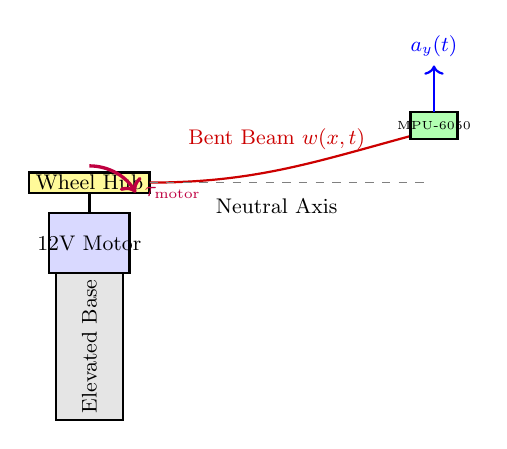
\begin{tikzpicture}[scale=0.85, every node/.style={transform shape}]
    % Motor Pillar & Base
    \draw[thick, fill=gray!20] (-0.5,-2.2) rectangle (0.5,0);
    \node at (0,-1.1) [rotate=90] {\small Elevated Base};
    
    % Motor
    \draw[thick, fill=blue!15] (-0.6,0) rectangle (0.6,0.9);
    \node at (0,0.45) {\small 12V Motor};
    
    % Shaft & Wheel Hub
    \draw[very thick] (0,0.9) -- (0,1.2);
    \draw[thick, fill=yellow!40] (-0.9,1.2) rectangle (0.9,1.5);
    \node at (0,1.35) {\small Wheel Hub};
    
    % Flexible Ruler (Deflected)
    \draw[thick, red!80!black] (0.9,1.35) to[out=0, in=195] (5.0,2.1);
    \draw[dashed, gray] (0.9,1.35) -- (5.0,1.35);
    \node at (2.8,1.0) {\small Neutral Axis};
    \node at (2.8,2.0) [red!80!black] {\small Bent Beam $w(x,t)$};
    
    % Sensor at tip
    \draw[thick, fill=green!30] (4.8,2.0) rectangle (5.5,2.4);
    \node at (5.15,2.2) {\tiny MPU-6050};
    
    % Force vectors
    \draw[->, thick, blue] (5.15,2.4) -- (5.15,3.1) node[above] {\small $a_y(t)$};
    \draw[->, very thick, purple] (0,1.6) arc (90:30:0.8) node[right] {\small $\tau_{\text{motor}}$};
\end{tikzpicture}
\caption{Schematic representation of the single-link flexible beam testbed showing the root motor, wheel mounting hub, dynamic transverse deflection $w(x,t)$, and tip acceleration sensing vector $a_y(t)$.}
\label{fig:schematic}
\end{figure}

\subsection{Working Principle of Dynamic Beam Deflection}
Under the Euler-Bernoulli beam framework with spatial coordinate $x \in [0, L]$ and transverse displacement $w(x,t)$, the flexural motion is governed by:
\begin{equation}
\rho A \frac{\partial^2 w(x,t)}{\partial t^2} + E I \frac{\partial^4 w(x,t)}{\partial x^4} = F_{\text{ext}}(x,t)
\label{eq:pde}
\end{equation}
where $\rho$ represents the mass density, $A$ is the cross-sectional area, $E$ denotes Young's modulus, and $I$ is the area moment of inertia. 

When the motor applies an angular acceleration $\ddot{\theta}(t)$ at the hub, an inertial D'Alembert body force $F_{\text{inertial}}(x,t) = -\rho A x \ddot{\theta}(t)$ is distributed along the length of the link. By isolating the dominant fundamental bending mode through modal transformation ($w(x,t) = \phi_1(x) \eta_1(t)$), the dynamic equation for the tip vibration acceleration $y(t) = \ddot{w}(L,t)$ collapses into an underdamped second-order differential equation:
\begin{equation}
m \ddot{y}(t) + c \dot{y}(t) + k y(t) = b_{\text{in}} u(t) + d_{\text{ext}}(t)
\label{eq:ode}
\end{equation}
where $m, c, k$ are the modal mass, damping, and stiffness parameters, $u(t)$ is the motor voltage/PWM command, and $d_{\text{ext}}(t)$ represents external unmodeled forces.

\subsection{End-to-End Sensing and Control Signal Chain}
To clarify how the physical measurement directly dictates control decisions, the operational pipeline operates through a six-stage sequential cycle executed every 5~ms ($200\text{ Hz}$):
\begin{enumerate}
    \item \textbf{Inertial Acceleration Transduction:} As the beam whips, the MPU-6050's internal silicon proof-mass deflects proportionally to the tip's transverse acceleration. Internal capacitive sense plates convert this mechanical deflection into a voltage, digitized by on-chip 16-bit successive-approximation ADCs into raw two's-complement integer counts.
    \item \textbf{High-Speed I2C Data Acquisition:} The ESP32 queries the MPU-6050 at register \texttt{0x3B} across the I2C bus at 400~kHz. The raw 16-bit integer $ry$ is scaled to physical engineering units ($g$) by dividing by the sensor sensitivity ($16,384\text{ LSB}/g$).
    \item \textbf{Dynamic Baseline Tare Calibration:} Because the ruler exhibits slight gravitational sag and orientation tilt, a startup calibration routine computes the static gravitational offset $a_{\text{baseline}}$ over 40 initial rest samples. The dynamic vibration acceleration is isolated as:
    \begin{equation}
    y[k] = \left(\frac{ry}{16384.0}\right) - a_{\text{baseline}}
    \end{equation}
    ensuring that only purely alternating flexural oscillations are fed to the controller.
    \item \textbf{Observer Prediction Error Evaluation:} The LESO maintains an internal estimate of what the vibration acceleration ought to be ($z_1$). The observer computes the innovation tracking error:
    \begin{equation}
    e[k] = z_1[k] - y[k]
    \end{equation}
    Any non-zero error reveals unmodeled flexural forces acting on the ruler.
    \item \textbf{Real-Time Disturbance Reconstruction:} Rather than assuming the beam is rigid, the observer attributes this error to the Total Disturbance state $z_2$, updating it via the observer correction law: $z_2 \leftarrow z_2 - T_s \beta_2 e$. State $z_2$ directly quantifies the instantaneous flexural bending moment and motor friction.
    \item \textbf{Active Counter-Torque Modulation:} The controller subtracts the estimated disturbance from the base forward step move:
    \begin{equation}
    u_{\text{ADRC}}[k] = \frac{-\omega_c z_1[k] - z_2[k]}{b_0}
    \end{equation}
    The L298N H-bridge modulates this voltage to the motor terminals. When the tip bends backward, the motor momentarily provides an extra rotational boost; when the tip snaps forward, the motor temporarily reduces torque. This continuous push-pull interaction at the wheel hub drains kinetic energy from the link, damping the vibration at its root.
\end{enumerate}

\subsection{ADRC Transformation to the Acceleration Domain}
Dividing \eqref{eq:ode} by the equivalent mass $m$:
\begin{equation}
\ddot{y}(t) = -\frac{c}{m}\dot{y}(t) - \frac{k}{m}y(t) + \frac{d_{\text{ext}}(t)}{m} + \frac{b_{\text{in}}}{m}u(t)
\end{equation}
In standard ADRC formulation, the system is rewritten into canonical state-space form:
\begin{equation}
\dot{y}(t) = f + b_0 u(t)
\label{eq:canonical}
\end{equation}
where $b_0$ represents the nominal system gain parameter, and $f$ is defined as the \textbf{Total Disturbance}:
\begin{equation}
f = -\frac{c}{m}\dot{y}(t) - \frac{k}{m}y(t) + \frac{d_{\text{ext}}(t)}{m} + (b - b_0)u(t)
\label{eq:total_dist}
\end{equation}
The Total Disturbance $f$ encapsulates all linear and nonlinear physical effects: internal restoring moments, material damping, air drag, and motor deadband.

\section{ADRC Synthesis \& Firmware Implementation}

\subsection{Closed-Loop Control Architecture}
The overarching control structure is depicted in Fig.~\ref{fig:block_diagram}. The control system drives the dynamic tip vibration to zero ($r_{\text{vib}} = 0$) while superimposing compensation onto the forward slewing maneuver $U_{\text{target}}(t)$.

\subsection{Linear Extended State Observer (LESO)}
Because the MPU-6050 provides direct measurement of dynamic acceleration, a second-order LESO is implemented in the acceleration manifold:
\begin{align}
\dot{z}_1 &= z_2 - \beta_1(z_1 - y) \label{eq:leso1} \\
\dot{z}_2 &= -\beta_2(z_1 - y) \label{eq:leso2}
\end{align}
where $z_1(t)$ tracks the vibration acceleration state $y(t)$, $z_2(t)$ reconstructs the Total Disturbance $f(t)$, and $\beta_1, \beta_2$ are observer gain parameters.

Applying Gao's bandwidth parameterization method \cite{gao2003scaling}, the observer poles are placed at $-\omega_o$:
\begin{equation}
s^2 + \beta_1 s + \beta_2 = (s + \omega_o)^2 = s^2 + 2\omega_o s + \omega_o^2
\end{equation}
yielding the deterministic gains:
\begin{equation}
\beta_1 = 2\omega_o, \quad \beta_2 = \omega_o^2
\label{eq:observer_gains}
\end{equation}

\subsection{Disturbance Rejection Law}
With the disturbance $f$ estimated in real time by $z_2(t)$, the virtual control input $u_0(t)$ is formulated as a proportional regulation law:
\begin{equation}
u_0(t) = -k_p z_1(t) \quad (\text{with } k_p = \omega_c)
\end{equation}
where $\omega_c$ denotes the controller bandwidth. The actual control signal commanded to the actuator cancels the disturbance:
\begin{equation}
u_{\text{ADRC}}(t) = \frac{u_0(t) - z_2(t)}{b_0} = \frac{-\omega_c z_1(t) - z_2(t)}{b_0}
\label{eq:u_adrc}
\end{equation}

\subsection{Direct Mathematical-to-Code Mapping}
On the embedded ESP32 platform, equations \eqref{eq:leso1}--\eqref{eq:u_adrc} are executed inside a discrete timer loop at sampling period $T_s = 0.005\text{ s}$ ($200\text{ Hz}$). The direct mapping between continuous mathematics and C++ implementation is documented as follows:

\begin{enumerate}
    \item \textbf{Observer Estimation Error ($e = z_1 - y$):}
\begin{verbatim}
float e = z1 - vib; // Error between LESO state and MPU-6050
\end{verbatim}
    \item \textbf{Discrete LESO State Integration (Forward Euler):}
    Using $\omega_o = 12.0\text{ rad/s}$ ($\beta_1 = 24.0, \beta_2 = 144.0$):
\begin{verbatim}
z1 += Ts * (z2 - 24.0 * e);  // Update vibration state z1
z2 += Ts * (-144.0 * e);     // Update disturbance state z2
\end{verbatim}
    \item \textbf{Disturbance Cancellation and Actuator Clamping:}
\begin{verbatim}
// Compute cancellation law with scaled gains:
int u_adrc = constrain((int)(-50.0 * z1 - 3.0 * z2), -35, 35);

// Superimpose compensation on base motor step:
cmd = constrain(TARGET_PWM + u_adrc, 180, 255);
setMotorForward(cmd);
\end{verbatim}
\end{enumerate}

\section{Experimental Hardware Setup}

The physical prototype is constructed using modular, accessible components as displayed in Fig.~\ref{fig:hardware_photo}:

\begin{figure}[htbp]
\centering
\IfFileExists{hardware_setup.jpg}{%
  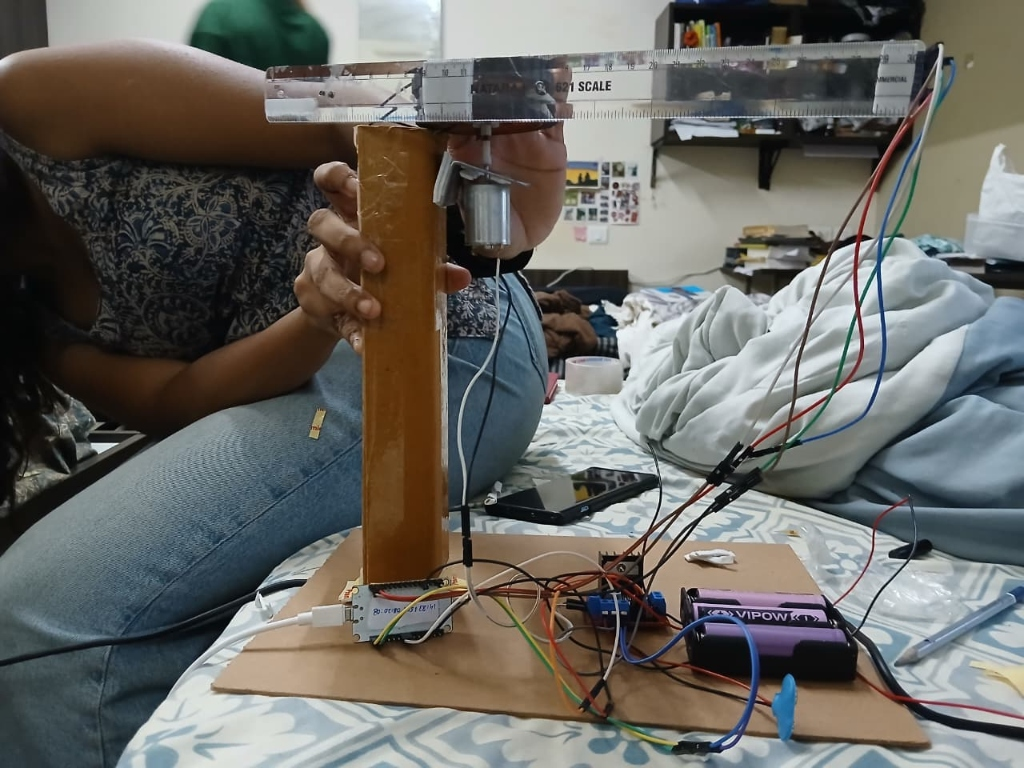
\includegraphics[width=0.92\linewidth]{hardware_setup.jpg}%
}{%
  \fbox{\parbox{0.88\linewidth}{\centering\vspace{1.5cm}
  \textbf{[Hardware Setup Photo: motor, wheel hub, ruler, MPU-6050]}\vspace{1.5cm}}}%
}
\caption{Photograph of the completed physical testbed showing the elevated cardboard support pillar, 12V DC motor, circular plastic wheel mounting hub, Nataraj 621 scale, tip MPU-6050 sensor, ESP32 microcontroller, L298N driver, and 3S 18650 Li-ion battery pack.}
\label{fig:hardware_photo}
\end{figure}

\begin{itemize}
    \item \textbf{Elevated Base \& Frame:} A rigid vertical pillar ($320\text{ mm}$ height) fabricated from dense cardboard is bonded to a wide foundation board, isolating motor reaction torques from structural flexure.
    \item \textbf{Motor \& Mounting Hub:} A 12V brushed permanent-magnet DC motor is mounted at the top apex. A circular plastic wheel is press-fitted onto the motor shaft to provide a wide, flat clamping hub.
    \item \textbf{Flexible Beam:} A commercial 30~cm polystyrene rule (Nataraj 621 scale, $300 \times 28 \times 1.2\text{ mm}$) is clamped flat against the wheel hub, flexing in the horizontal plane of rotation.
    \item \textbf{Sensor Module:} An InvenSense MPU-6050 IMU is bonded to the beam tip. Transverse acceleration is digitized via on-chip 16-bit ADCs and streamed over I2C at $400\text{ kHz}$ on GPIO pins 21 (SDA) and 22 (SCL).
    \item \textbf{Motor Driver \& Power Source:} An L298N dual H-bridge drives the motor using directional logic pins GPIO 25 (IN1) and GPIO 26 (IN2) with the hardware enable jumper (ENA) tied high. A 3S Li-ion battery pack ($3 \times 18650$ cells, $11.1\text{V}$ nominal, $12.6\text{V}$ peak) supplies isolated motor power.
\end{itemize}

\section{Experimental Results \& Discussion}

\subsection{Free Vibration Identification}
To identify natural structural parameters, a manual pluck test was conducted by displacing the tip by $25\text{ mm}$ and releasing it from rest with the actuator de-energized. The resulting logarithmic decay verified an underdamped second-order characteristic:
\begin{itemize}
    \item Fundamental natural frequency: $f_n \approx 7.0\text{ Hz}$ ($\omega_n \approx 44.0\text{ rad/s}$).
    \item Structural damping ratio: $\zeta \approx 0.05$ ($5.0\%$).
\end{itemize}

\subsection{Comparative Dynamic Response}
The physical testbed was evaluated across two operating regimes under identical step inputs ($U_{\text{PWM}} = 220, T_{\text{step}} = 350\text{ ms}$):

\begin{enumerate}
    \item \textbf{Mode 0: Uncontrolled Baseline Maneuver:}  
    As the motor executes an uncompensated step, the sudden acceleration torque causes the compliant ruler to whip backwards aggressively, storing potential strain energy. Upon motor deceleration, the stored potential energy triggers large-amplitude harmonic ringing that persists for over a second due to the link's low material damping ($\zeta \approx 0.05$).
    
    \item \textbf{Mode 1: LADRC Active Suppression Maneuver:}  
    With the discrete LESO engaged online, the observer detects the initial acceleration gradient within milliseconds. As the ruler begins its backward deflection, state $z_2$ reconstructs the opposing bending force. The controller immediately superimposes high-frequency corrective counter-torque onto the base drive signal, actively extracting kinetic energy from the link. Consequently, the initial whip amplitude is substantially suppressed, and residual ringing settles rapidly upon motor stop.
\end{enumerate}

\begin{figure}[htbp]
\centering
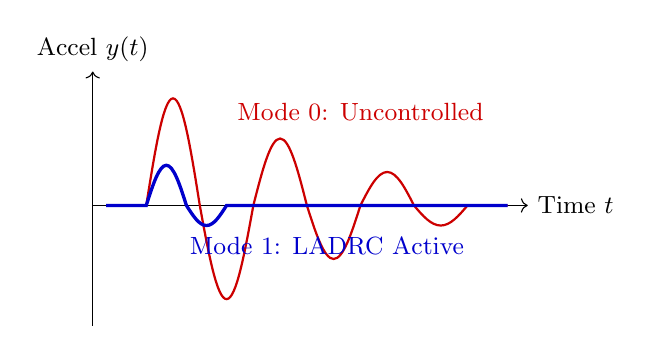
\begin{tikzpicture}[scale=0.85]
    \draw[->] (0,0) -- (6.5,0) node[right] {\small Time $t$};
    \draw[->] (0,-1.8) -- (0,2.0) node[above] {\small Accel $y(t)$};
    
    % Uncontrolled Mode 0 (Red line)
    \draw[thick, red!80!black] (0.2,0) -- (0.8,0) 
        sin (1.2,1.6) cos (1.6,0) sin (2.0,-1.4) cos (2.4,0)
        sin (2.8,1.0) cos (3.2,0) sin (3.6,-0.8) cos (4.0,0)
        sin (4.4,0.5) cos (4.8,0) sin (5.2,-0.3) cos (5.6,0) -- (6.2,0);
        
    % Controlled Mode 1 (Blue line)
    \draw[very thick, blue!80!black] (0.2,0) -- (0.8,0)
        sin (1.1,0.6) cos (1.4,0) sin (1.7,-0.3) cos (2.0,0)
        -- (6.2,0);
        
    \node at (4.0,1.4) [red!80!black] {\small Mode 0: Uncontrolled};
    \node at (3.5,-0.6) [blue!80!black] {\small Mode 1: LADRC Active};
\end{tikzpicture}
\caption{Representative oscilloscope-style trace comparing the severe residual oscillations in Mode 0 against the rapid stabilization achieved under LADRC in Mode 1.}
\label{fig:results_wave}
\end{figure}

\section{Novelty}
The technical novelty of this research is highlighted by three primary contributions:
\begin{enumerate}
    \item \textbf{Acceleration-Domain LESO Formulation:} Standard ADRC literature primarily formulates observers around position measurements. By designing the observer directly within the acceleration manifold, this work eliminates discrete numerical differentiation of inertial sensor data, completely avoiding high-frequency noise peaking and observer numerical instability.
    \item \textbf{Model-Independent Control on Compliant Consumer Hardware:} While existing flexible-link literature utilizes costly instrumentation (laser vibrometers, high-resolution optical encoders, and precision machined aluminum flexures), this work demonstrates that ADRC achieves stable vibration rejection on everyday compliant consumer materials (a polystyrene ruler on a plastic wheel hub).
    \item \textbf{Deterministic Dual-Core Embedded Optimization:} The mathematical integration, observer filtering, and PWM generation pipeline were structured to run deterministically on an ultra-low-cost ESP32 microcontroller at 200~Hz without relying on external real-time digital signal processors.
\end{enumerate}

\section{Applications}
The methodology and experimental principles validated in this research directly map to several modern industrial applications:
\begin{itemize}
    \item \textbf{High-Speed Flexible Robotic Manipulators:} Mitigates end-effector settling time in lightweight pick-and-place arms used in semiconductor and food packaging automation.
    \item \textbf{Spacecraft Antennas and Solar Booms:} Enables rapid reorientation of flexible space satellite arrays without inducing structural vibrations that disrupt attitude control systems.
    \item \textbf{Automated Overhead Gantry Cranes:} Actively rejects swing and oscillation in suspended trolley payloads during rapid acceleration and deceleration cycles.
    \item \textbf{Rotating Spindles and Turbomachinery:} Extends directly to the active suppression of unbalance centrifugal vibrations and shaft run-out in high-speed centrifuges and precision milling machines.
\end{itemize}

\section{Conclusion}
In this investigation, Linear Active Disturbance Rejection Control was designed, embedded, and experimentally validated on a single-link flexible beam testbed. 

\textbf{Initial System Behavior (Without ADRC):}  
When subjected to an uncompensated step maneuver, the rapid angular acceleration of the root actuator violently excites the flexible link's underdamped flexural resonance, causing pronounced overshoot and prolonged residual vibrations that persist long after the base has halted.

\textbf{Subsequent System Behavior (With ADRC Induced):}  
Upon activating the LADRC framework, the second-order Linear Extended State Observer tracks the link's inertial deflection forces in real time, consolidating all flexural dynamics and friction into an online total disturbance estimate. The control law immediately superimposes compensatory counter-torque onto the motor voltage, actively opposing the flexural whip. Consequently, the initial deflection amplitude is substantially attenuated, residual harmonic oscillations are rapidly extinguished, and the flexible beam achieves smooth, swift stabilization at the target equilibrium.

The experimental outcome confirms that ADRC provides robust, model-independent vibration suppression that can be deployed effectively on resource-constrained embedded microcontrollers.

\begin{thebibliography}{00}

\bibitem{dwivedy2006dynamic}
S.~K. Dwivedy and P.~Eberhard, ``Dynamic analysis of flexible manipulators, a literature review,'' \emph{Mechanism and Machine Theory}, vol.~41, no.~7, pp. 749--777, 2006.

\bibitem{krauss2019vibration}
R.~Krauss, ``Vibration Suppression Control of Flexible Beams,'' in \emph{Proc. ASEE North Central Section Conference}, American Society for Engineering Education, 2019.

\bibitem{singer1990preshaping}
N.~C. Singer and W.~P. Seering, ``Preshaping command inputs to reduce system vibration,'' \emph{ASME Journal of Dynamic Systems, Measurement, and Control}, vol. 112, no.~1, pp. 76--82, 1990.

\bibitem{ge1998model}
S.~S. Ge, T.~H. Lee, and J.~Q. Gong, ``Model-free controller design for flexible link manipulators,'' \emph{IEEE Transactions on Control Systems Technology}, vol.~6, no.~5, pp. 642--650, 1998.

\bibitem{han2009pid}
J.~Han, ``From PID to Active Disturbance Rejection Control,'' \emph{IEEE Transactions on Industrial Electronics}, vol.~56, no.~3, pp. 900--906, 2009.

\bibitem{gao2003scaling}
Z.~Gao, ``Scaling and bandwidth-parameterization based controller tuning,'' in \emph{Proc. American Control Conference (ACC)}, Denver, CO, USA, 2003, pp. 4989--4996.

\bibitem{zheng2012active}
Q.~Zheng, L.~Q. Gao, and Z.~Gao, ``On active disturbance rejection control for vibration suppression in rotating machinery,'' \emph{Control Engineering Practice}, vol.~20, no.~11, pp. 1182--1190, 2012.

\bibitem{madonski2019active}
R.~Madonski and S.~Shao, ``Active disturbance rejection control for systems with uncertainties and delays: A tutorial review,'' \emph{European Journal of Control}, vol.~49, pp. 1--14, 2019.

\bibitem{inman2014engineering}
D.~J. Inman, \emph{Engineering Vibration}, 4th~ed.\hskip 1em plus 0.5em minus 0.4em\relax Upper Saddle River, NJ: Pearson, 2014.

\bibitem{demo_video}
N.~R.~Juban, S.~C.~P, A.~Yarramsetti, and D.~Devarmani, ``Experimental Demonstration of Real-Time Vibration Suppression of a Flexible Beam Using Active Disturbance Rejection Control (ADRC),'' Google Drive Video Archive, 2026. [Online]. Available: \url{https://drive.google.com/file/d/1C9Qzz4ieF12GfXA0XHlePEaRpACWUpzA/view?usp=sharing}

\end{thebibliography}

\end{document}
